\section{Topology\label{sec:topology}}

The XK-XMP-64 connects together 64 XCore processors in 16 XS1-G4 devices. These
are arranged as a 4-dimensional \emph{hypercube} using 5b XMOS links on a single
PCB. A hypercube is a generalisation of a regular cube structure into an
arbitrary number of dimensions. A $d$-dimensional hypercube is a special case of
a $k$-ary $n$-cube (torus network) when $k = 2$, and has $N = 2^d$ nodes and
$d2^{d-1}$ edges. Each node in the network can be labeled with a $d$-bit binary
identifier, and an edge exists between two nodes $x$ and $y$ if and only if
their identifiers differ by exactly one bit, i.e.\ for some integer $k\geq0$
$$x\oplus y=2^k.$$ Hence, each node has $d = \log N$ edges. An edge is called a
\emph{dimension $e$ edge} if it links two nodes whose identifiers differ in the
$e$\textsuperscript{th} bit position \cite{leighton92}.

Intuitively, a $4$-dimensional hypercube can be constructed by joining two cube
structures (each with $8$ nodes), by adding edges between corresponding
vertexes.  Figure \ref{fig:hypercube} illustrates this.  Incidentally, a $4$-ary
$2$-cube is equivalent to a $4$-dimensional hypercube, and this \emph{flat}
structure is used to package the hypercube network between the 16 chips in the
XK-XMP-64. As each chip contains 4 cores, it is convenient to view the network
as a hypercube with 6 dimensions. 

\begin{figure}[ht]
\centering
\subfloat[]{
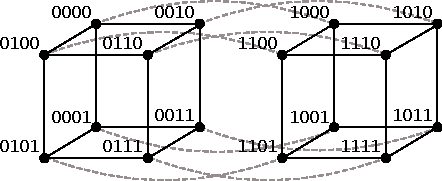
\includegraphics[scale=1]{../images/hypercube.pdf}
\label{fig:hcubea}
}
\hspace{10mm}
\subfloat[]{
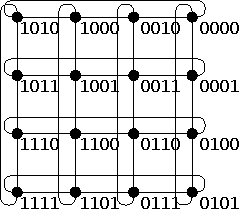
\includegraphics[scale=1]{../images/torus.pdf}
\label{fig:hcubeb}
}
\caption{Representations of a 4-dimensional hypercube. \protect\subref{fig:hcubea}
shows an intuitive construction and \protect\subref{fig:hcubeb} shows an equivalent
$4$-ary $2$-cube, or torus network, which is used to package the hypercube on
the XMP-64 board.}
\label{fig:hypercube}
\end{figure}

